\documentclass[11pt,a4paper]{article}
\usepackage{amsmath}
\usepackage{graphicx}
\usepackage[acronym]{glossaries}
\graphicspath{ {\string~/Desktop/} }
\usepackage[left=2.54cm, right=2.54cm, top=2.54cm]{geometry}
\usepackage{indentfirst}
\usepackage{fontspec}
\setmainfont{Arial}
\usepackage{url}
\usepackage{notoccite}
\setlength\parindent{1cm}
\usepackage{titlesec}
\titlelabel{\thetitle.\quad}
\usepackage{caption}
\usepackage{subcaption}
\captionsetup[figure]{font=small}
\usepackage{breakcites}

\title{Robust Resource Allocation Model Using Edge Computing for Delay Sensitive Tasks in Vehicle to Infrastructure (V2I) Networks}
\date{}

\begin{document}
\maketitle
\newacronym{bs}{BS}{Base Station}
\newcommand{\ie}{\textit{i}.\textit{e}.,}
\newcommand{\eg}{\textit{e}.\textit{g}.,}
\newcommand{\bs}{\text{Base Station}}

\begin{center}
\textbf{Anna Kovalenko\textsuperscript{1}, Razin Farhan Hussain\textsuperscript{2}, Mohsen Amini Salehi\textsuperscript{3} and Omid Semiari\textsuperscript{4}}
\small{High Performance Cloud Computing (HPCC) Lab. School of Computing and Informatics, University of Louisiana at Lafayette Louisiana, USA. aok8889@louisiana.edu} \\
\small{High Performance Cloud Computing (HPCC) Lab. School of Computing and Informatics, University of Louisiana at Lafayette Louisiana, USA. razinfarhan.hussain1@louisiana.edu} \\
\small{High Performance Cloud Computing (HPCC) Lab. School of Computing and Informatics, University of Louisiana at Lafayette Louisiana, USA. amini@louisiana.edu} \\
\small{Department of Electrical and Computer Engineering, Georgia Southern University Georgia, USA. osemiari@georgiasouthern.edu}
\end{center}


\section*{\normalsize\uppercase{Abstract}}
Development of autonomous vehicles is one of the most ambitious and promising projects in human history. Such vehicles require agile and reliable services to manage hazardous road situations. Vehicular Networks is the technology that can provide high-quality services for self-driving vehicles. A large percentage of service requests in these networks have an urgent nature (\eg \ disaster updates, hazard alerts, etc.) In other words, these requests are delay intolerant and require immediate service. Therefore, Vehicular Networks, and particularly, Vehicle-to-Infrastructure (V2I) systems must provide a consistent real-time response to autonomous vehicles. During increased traffic congestion or even natural disasters, it can be particularly tricky for V2I systems to maintain an optimal performance level. In such situations, a surge of requests arriving at a \bs \ (a network edge device with computing capabilities) can drastically decrease V2I system response time. The consequences of even a millisecond delay for an urgent request can be dangerous, sometimes fatal. Hence, the goal of our research is to increase robustness (\ie \ ability to maintain optimal performance) of the V2I systems. To achieve this goal, we offer a resource allocation model that can load balance (\ie \ dynamically utilize resources from neighboring \bs s), when the system is oversubscribed (experiencing an unusually dense service requests arrival). We propose an allocation algorithm based on a calculated probability of the arriving request to be served in time on several neighboring \bs s. We introduce a Load Balancer component which assigns the request to the \bs \ with a maximum precomputed probability. After all, we evaluate our model under various oversubscription levels and urgent requests percentages. Simulation results demonstrate that the proposed model decreases overall service miss rate by up to 20 \% and urgent requests miss rate by up to 50 \%. \\

{\bf Keywords:} Vehicular Networks, V2I, Edge Computing, High Performance.


\section*{\normalsize\uppercase{1. Introduction}}\label{sec:intro}
Recent advancements in communication and computation technologies have stimulated a rapid development of vehicular networks. Federal Communications Commission (FCC) has reserved 5.850 to 5.925 GHz frequency band for Vehicle-to-Everything (V2X) communications~\cite{ali2011co}. Vehicle-to-Infrastructure (V2I) communications is one prominent form of V2X that draws the majority of work to itself. In V2I, infrastructure refers to all edge and core technologies that facilitate communications and computations for vehicular requests.

As shown in Figure~\ref{fig:scen}, autonomous vehicles send their service requests (tasks) to Base Stations while operating on the road. A \bs \ is capable of communicating with vehicles and processing vehicular tasks~\cite{bok2016multiple}. Upon the completion of the processing, the results sent back to the requesting vehicle. Examples of such vehicular tasks can be a Wrong Way Driver warning~\cite{ABIresearch}, Cooperative Forward Collision warning~\cite{ElBatt}, and Lane Change warning~\cite{ABIresearch}. This type of tasks can only tolerate a short end-to-end delay~\cite{ali2011co}. For such delay-sensitive requests, there is no value in executing them after a tolerable delay.


\begin{figure}[!h]
\centering
\includegraphics[scale=0.38]{scenario.png}
\caption{A Vehicle to Infrastructure (V2I) scenario where vehicles send requests to a Base Station and receive the response. A Base Station is a roadside unit with communicational and computational abilities.}
\label{fig:scen}
\end{figure}


Significant problems arise during road emergencies (\eg \ road accidents and disasters) when a rapid increase in service requests to \bs s significantly affects the tasks' service time. In fact, in this situation, \bs \ resources become oversubscribed, and it cannot provide enough computational power for all the arriving tasks to meet their deadlines. Accordingly, our goal, in this research, was to design the V2I system to be robust against uncertain task arrival. In the literature, \emph{robustness} is defined as the degree to which a system can maintain a certain level of performance even with given uncertainties \cite{ali2004measuring, smith2009robust, canon2010evaluation}. In our research, we evaluate robustness of the V2I system according to the number of tasks that can meet their deadlines. The main question we try to answer is how to allocate arriving tasks among the \bs s so that the system stays robust? Or, in other words, we try to find a way to maximize the number of tasks meeting their deadlines. 

Previous research works either discard these uncertainties~\cite{bok2016multiple} or focus on the uncertainty introduced by communication~\cite{ali2011co}. Alternatively, to assure robustness of the V2I system, we propose a probabilistic resource allocation model that copes with uncertainties introduced by both communication and computation. Our proposed model is aware of the connectivity amongst \bs s (\ie \ edge nodes) and their heterogeneity. In the face of oversubscription, we devise a Load Balancer at the \bs~level that can leverage the computational capabilities of other \bs s to improve robustness of the V2I system.

According to our model, when the task arrives to a \bs \ it enters the Load Balancer (Figure \ref{fig:model}). The Load Balancer works in an immediate mode to allocate arriving tasks to the \bs s. It can allocate the task to the receiving \bs \ or to the one-hop distance neighboring \bs. When the task is allocated, it enters the batch queue of the \bs \ to be scheduled for processing.

\begin{figure}[h]
\centering
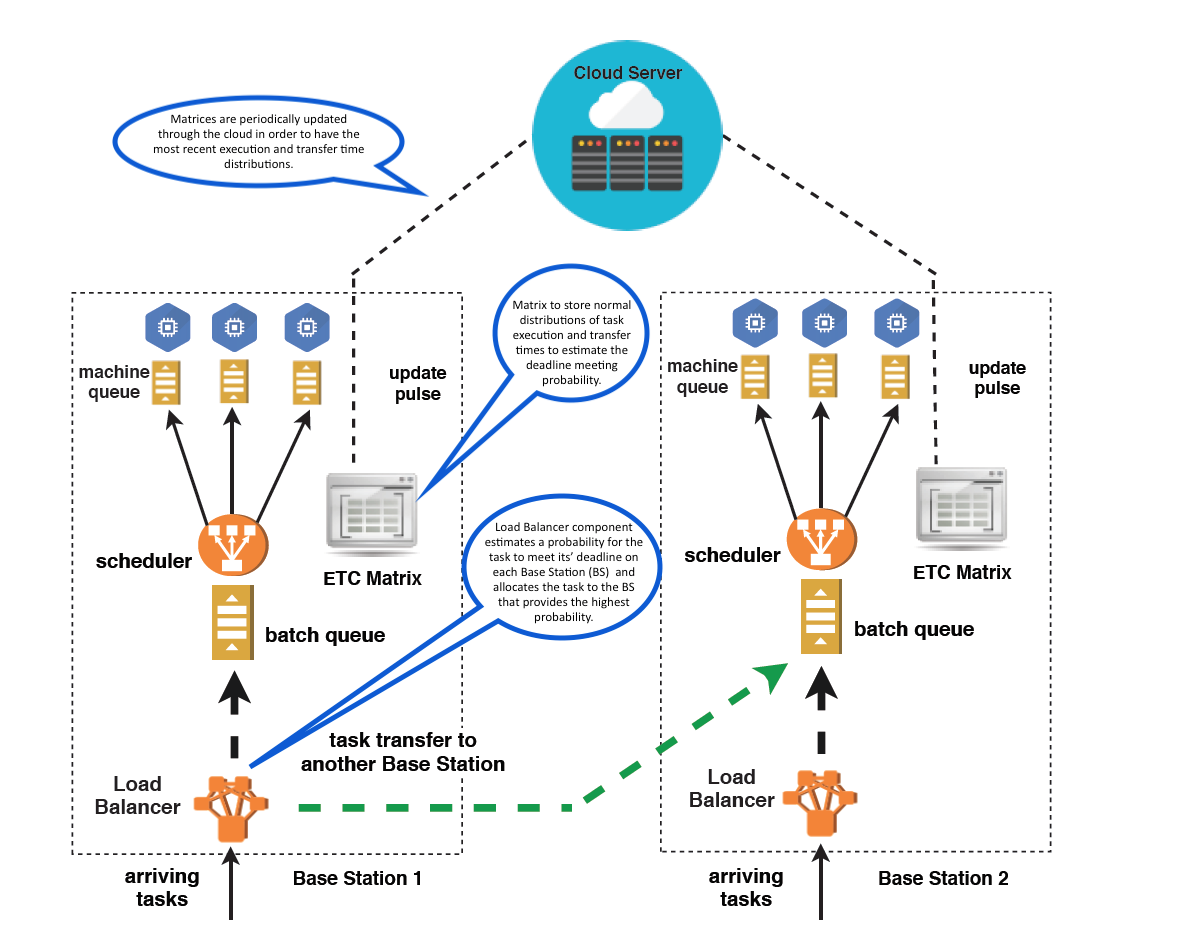
\includegraphics[scale=0.38]{model.png}
\caption{A proposed model where the task gets efficiently allocated by the Load Balancer between receiving and neighboring Base Stations.}
\label{fig:model}
\end{figure}

Every \bs \ stores two matrices (ETC Matrix component in Figure~\ref{fig:model}) to enable probability computation proposed in our model. One matrix is the Estimated Task Completion time (ETC) matrix~\cite{ali2000representing}. Another one is the Estimated Task Transfer time (ETT) matrix. These two matrices contain estimated task completion and task transfer time normal distributions (X$\sim \mathcal{N}(\mu,\,\sigma^{2})$) respectively. These distributions are based on historical execution and transfer times of different task types (delay tolerant and intolerant). Matrices are updated periodically through the cloud.

For each task $t_i$  of task type "i," Load Balancer calculates the probability ($P_i^j$) of this task to meet its deadline $\delta_i$ across the receiving and neighboring \bs s. For the receiving \bs \ "j", the probability can be defined as $P_i^j$($\gamma_i^j$ \textless $\delta_i$ ) = $P_i^j$(Z \textless z) where "z" is ($\delta_i$- $\mu_i^j$) / $\sigma_i^j$. We standardize the distribution with $\mu_i$ = 0 and $\sigma_i$ = 1. For all of the neighboring \bs s, to calculate the probability, Load Balancer convolves the ETC distribution with respective ETT distribution. The convolution is necessary to account for the transfer time to a neighboring \bs. 
The resulting distribution (W$\sim \mathcal{N}(\mu,\,\sigma^{2})$) is used to calculate the probability of the task meeting the deadline in a specific \bs. If a neighboring \bs \ is "k" and task type is "i" then the probability can be defined as "$P_i^k$" where z = ($\delta_i$ - $\mu_i^k$) / $\sigma_i^k$. When the probability of the received task in all of the \bs s (receiving and neighboring) is calculated, the task gets allocated to the \bs \ that offers the highest probability. When the task's probability to meet its deadline is zero (0), the task is dropped (it will not enter any batch queue for scheduling). Task dropping procedure during the oversubscription situation implicitly increases the probability of the other tasks to meet their deadlines.

The results of our research prove that the proposed model offers a better, more robust allocation algorithm. We evaluate our model using EdgeCloudSim simulation~\cite{cloudsim}. Our resource allocation model is tested against the Baseline model. The Baseline model always allocates arriving task to a receiving \bs. Figure~\ref{fig:perf} represents simulation results of overall system performance for medium and high system oversubscription levels. Our model provides noticeably better results when the number of vehicles is less than or equal to 100. Otherwise, it's performance decreases as well as the Baseline's performance. Regardless, our system consistently performs 2-5 \% better than the Baseline. 

\begin{figure}[h]
\centering
\begin{subfigure}{.5\textwidth}
  \centering
  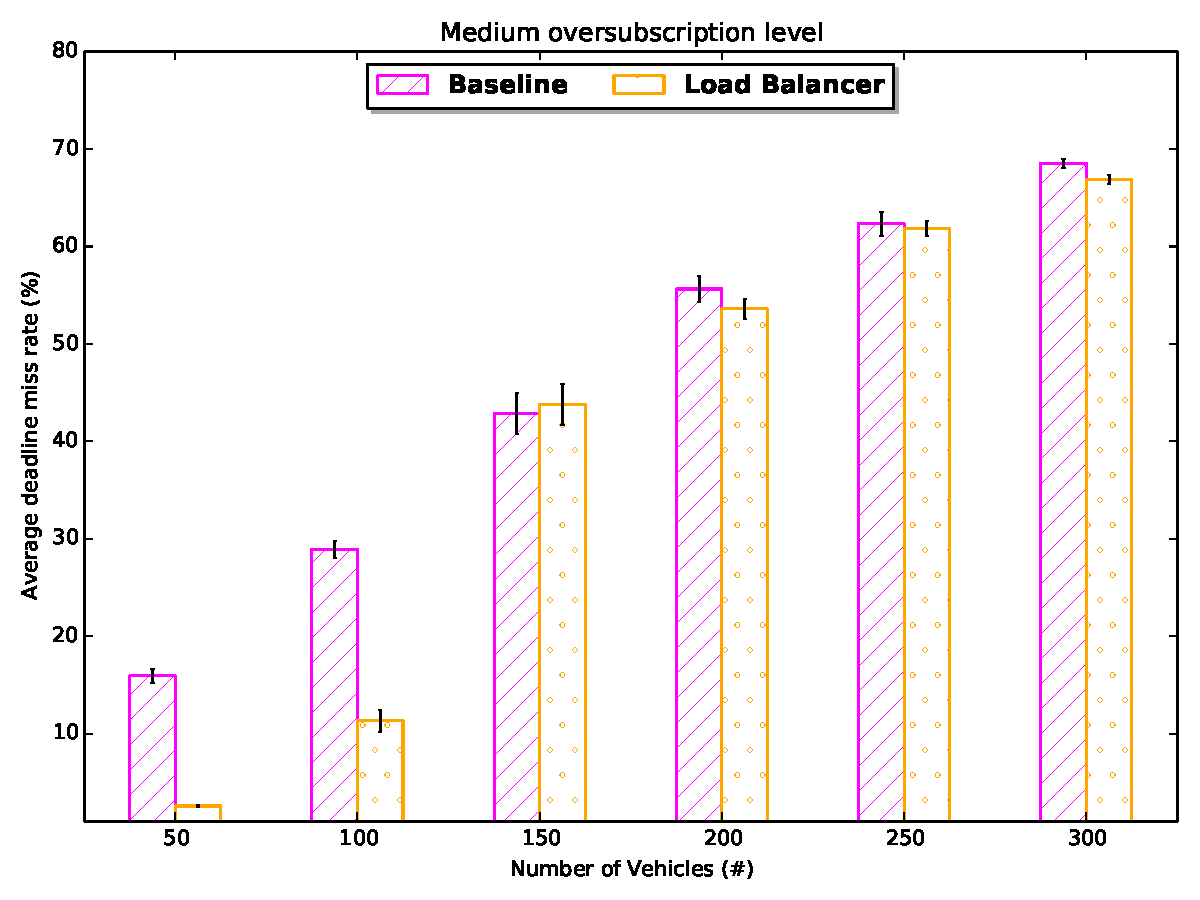
\includegraphics[scale=0.38]{20min.pdf}
\end{subfigure}%
\begin{subfigure}{.5\textwidth}
  \centering
  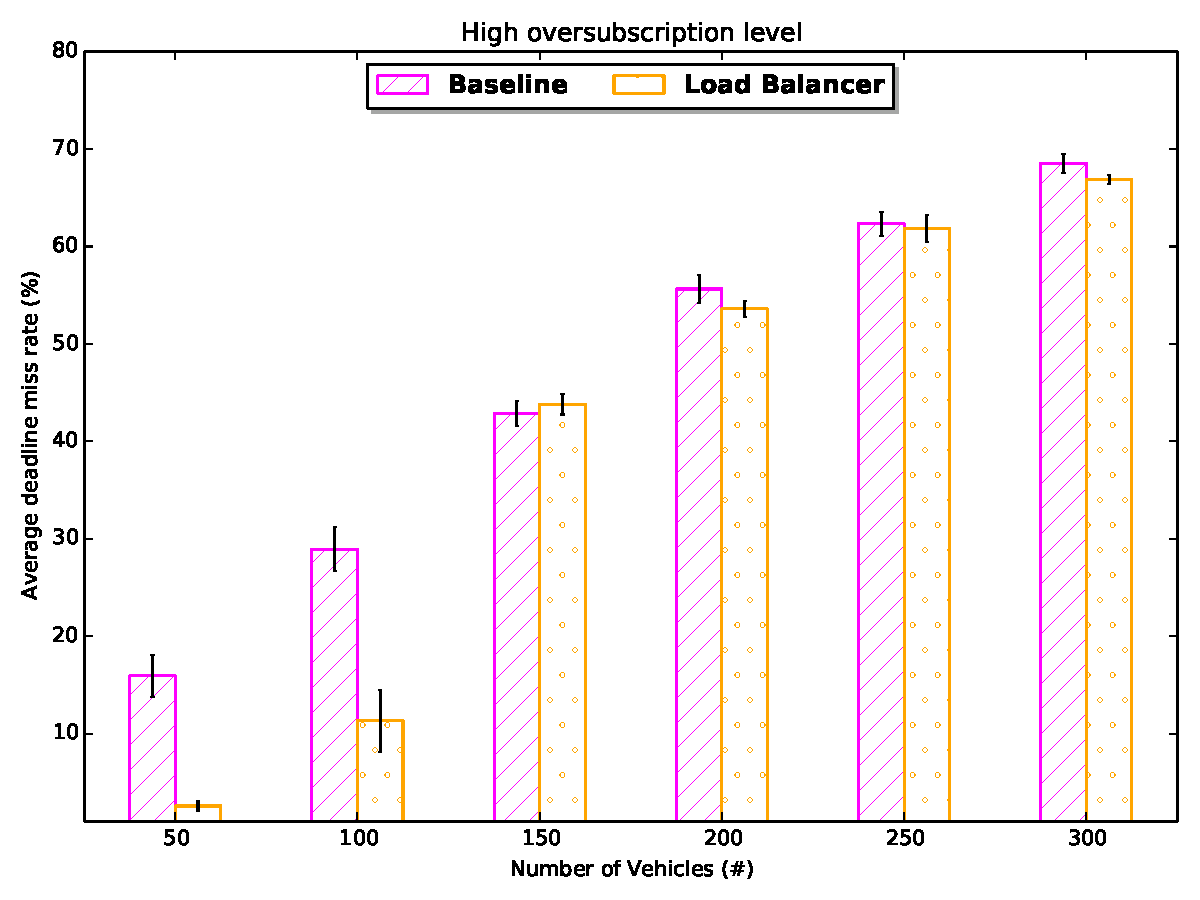
\includegraphics[scale=0.38]{10min.pdf}
\end{subfigure}
\caption{Load Balancer overall service miss rate compared to the Baseline.}
\label{fig:perf}
\end{figure}

\begin{figure}[h]
\centering
\begin{subfigure}{.5\textwidth}
  \centering
  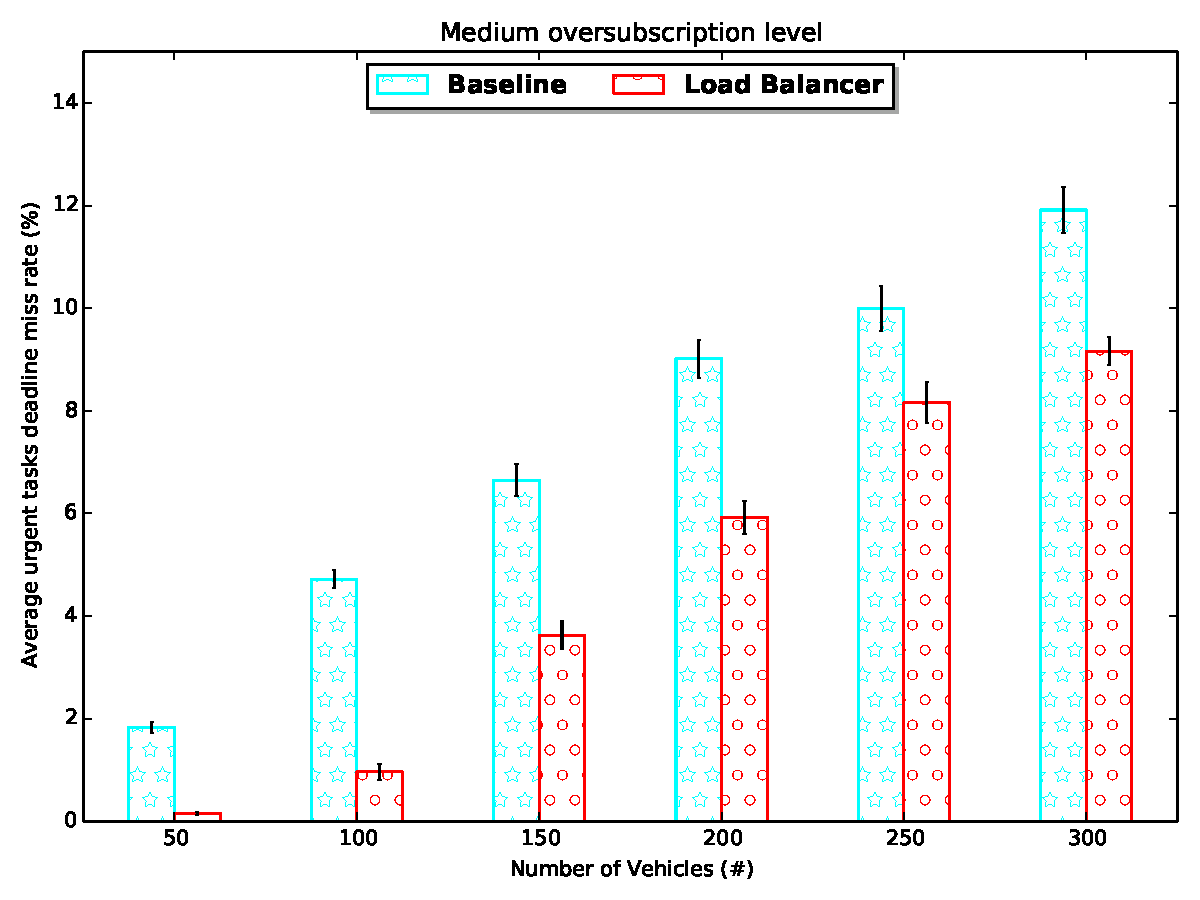
\includegraphics[scale=0.38]{20minU.pdf}
\end{subfigure}%
\begin{subfigure}{.5\textwidth}
  \centering
  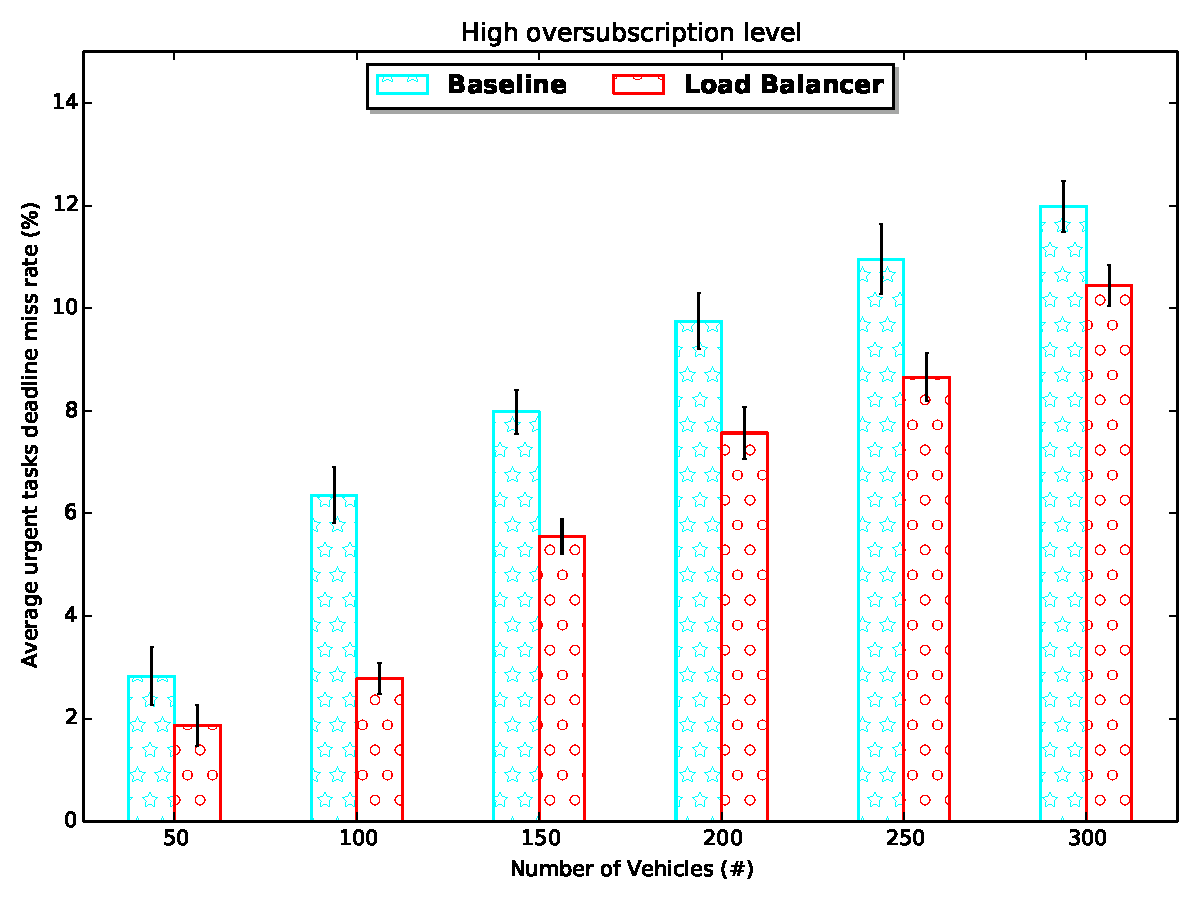
\includegraphics[scale=0.38]{5minU.pdf}
\end{subfigure}
\caption{Load Balancer urgent service miss rate compared to the Baseline.}
\label{fig:perfU}
\end{figure}

Nevertheless, the most crucial improvement our system presented in Figure 4. Our research aimed to provide a resource allocation model that would be robust against computational and communicational uncertainties, especially for the service requests that have an urgent nature. Figure 4 shows the deadline miss rates for urgent tasks both for our model and the Baseline. The left caption represents the performance for the medium level of oversubscription and the right one for the high. We can notice, that our proposed model consistently performs better than the Baseline. When the number of vehicles is low, Load Balancer allows for up to 80 \% improvement. With a more significant amount of vehicles up to 50 \% performance improvement is present.

Finally, I can conclude our research results to be successful. We proposed a model that encompasses the uncertainties exist in communication and computation. We developed a load balancing heuristic that increases the robustness of the V2I system. The analysis of the results confirms the success and allows to continue expanding our model, and possibly introducing a real-world implementation in the future. 

\bibliographystyle{apalike}
\bibliography{abstract}


\end{document}

%Related literature suggests incorporating wireless network infrastructure and cloud computing capabilities to enhance the performance of V2I systems~\cite{yu2016optimal}. For instance, the Vehicular Cloud Computing (VCC) was initiated in \cite{gerla2012} as a subsection of Mobile Cloud Computing. However, both VCC and conventional cloud systems incur high latency~\cite{li2017resource} thus, cannot be used for delay intolerant tasks. Nonetheless, \bs ' computational power can be harnessed with an edge computing system. With the edge device, vehicular services can be managed directly at the \bs \ with low latency and with no necessity to communicate with the cloud. Various \bs s in a V2I system can potentially be heterogeneous, both in terms of computational characteristics and communication medium to the core network (\eg \ wireless, optical, and wired \cite{bok2016multiple}). 
%Any possible solution to this problem needs to overcome the uncertainties of the system. In particular, uncertainty imposed by indeterministic task arrival rate and by the communication delay.